%==WORKSHEET 2

\newpage
\stepcounter{handout}
\begin{exercisebox}[adjusted title=Variables]
Create a new project (``File'' -> ``New'') and immediately save it
the project. Call it ``Aquarium''.\\
\\
\noindent
Type in this piece of code:

\begin{lstlisting}[language=JavaScript]
function setup() {
  createCanvas(400, 400);
  background(220);
  
  //basic fish shape
  fishX = 150;
  ellipse(fishX, 200, 120, 75);
  triangle(fishX - 60, 200, fishX - 90, 170, fishX - 90, 230);
}

function draw() {
 
}

\end{lstlisting}
Try changing 150 to a different number in the \ttpy{fishX} specification.

\noindent
Now add the following:
\begin{lstlisting}[language=JavaScript]
  eyeSize = 15;
  ellipse(fishX + 30, 190, eyeSize, eyeSize);
\end{lstlisting}
Try changing the value of \ttpy{eyeSize}.

\tcbsubtitle{Tasks:}
\noindent
You have now added a fish that can be moved just by changing one
value.

\begin{itemize}
\item Color the fish
\item Give the fish a fin that moves when you change \ttpy{fishX}.
\item Give the fish a pupil that moves when you change \ttpy{fishX}.
\item Create a new variable, \ttpy{fishY}, that controls the y-position of the fish
\end{itemize}

\hspace{1cm}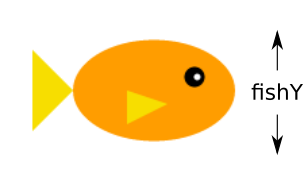
\includegraphics[width=0.4\textwidth]{illustrationer/fisk-fishY.png}

\noindent
Remember to save the project. We'll be working on it later.

\end{exercisebox}
\newpage
\begin{exercisebox}[adjusted title= Green City continues]
Switch to the electric car project and introduce variables to specify the
location of the objects so that we can later animate these objects.

\begin{itemize}
\item Create a variable \ttpy{carX} so the car can move forward
  and back
\item Create a variable \ttpy{cloudX} so the cloud can move back and forth
\item Create a variable \ttpy{treeX} so the tree can be moved horizontally
\item Create a variable \ttpy{treeY} so the tree can be moved vertically
\end{itemize}
\begin{center}
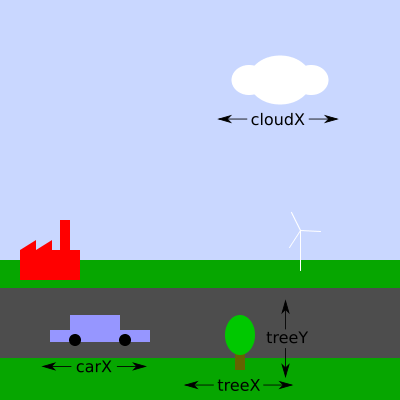
\includegraphics[width=0.5\textwidth]{illustrationer/carX-cloudX-treeXY.png}
\end{center}
\end{exercisebox}

\begin{exercisebox}[adjusted title=Aquarium Continues]
Use what you've learned to expand your aquarium project; here's an
example, but feel free to use your imagination! For example, one variable is used
for the x-coordinate of the seaweed plant and another variable for the x-coordinate
of the entire group of rocks (as a unit). An additional set of
variables \ttpy{fish2X}/\ttpy{fish2Y} to control the location of the
additional fish.%  Man kunne også forestille sig bobler, et mini sandslot,
% andre tangplanter, muslingeskaler eller andre dyr.

\begin{center}
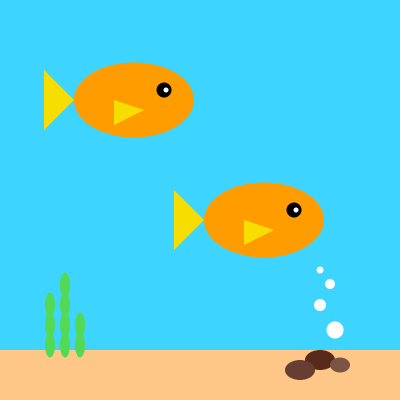
\includegraphics[width=0.4\textwidth]{illustrationer/akvarie.png}
\end{center}

\end{exercisebox}
